\chapter{\label{chap:related-work}Trabalhos Relacionados}
% MarI/O
% - https://www.youtube.com/watch?v=qv6UVOQ0F44 
% - https://www.youtube.com/watch?v=iakFfOmanJU 
% - https://www.youtube.com/watch?v=S9Y_I9vY8Qw 

% Atari DeepMind
% - http://arxiv.org/pdf/1312.5602v1.pdf 
% - https://storage.googleapis.com/deepmind-data/assets/papers/DeepMindNature14236Paper.pdf  

% NERO
% - http://nn.cs.utexas.edu/?stanley:ieeetec05 

\section{N.E.R.O: Neuro-Evolving Robotic Operatives}

\begin{mdframed}[backgroundcolor=green!20]
\begin{itemize}
    \item
        O que é
    \item
        Técnica utilizada (citar paper)
    \item
        Relevância com o nosso trabalho
\end{itemize}
\end{mdframed}

%----------
\section{Atari DeepMind}

\begin{mdframed}[backgroundcolor=green!20]
\begin{itemize}
    \item
        O que é
    \item
        Técnica utilizada (citar paper)
    \item
        Relevância com o nosso trabalho
\end{itemize}
\end{mdframed}

%----------
\section{MarI/O}

Em junho de 2015, o canal do \textit{YouTube}
SethBling\footnote{https://www.youtube.com/user/sethbling/about} -- conhecido
por publicar vídeos de modificações de jogos como Mario e Minecraft -- divulgou
o vídeo \textit{MarI/O - Machine Learning for Video
Games}\footnote{https://www.youtube.com/watch?v=qv6UVOQ0F44}, que mostra um
jogador muito habilidoso completando o nível \textit{Donut Plains I} de
\textit{Super Mario World}. É explicado, então, que o jogador em questão não é
humano, mas sim um programa de computador. Utilizando um emulador de
\textit{consoles} chamado \textit{BizHawk}, a linguagem de programação
\textit{Lua} e uma técnica de inteligência artificial chamada
\textit{\textbf{N.E.A.T}} (\textit{NeuroEvolution of Augmenting Topologies}), o
autor programou um \textit{bot} capaz de aprender como jogar o nível em questão
do início ao fim com sucesso. Como é explicado no vídeo, inicialmente o
\textit{bot} não conhecia absolutamente nada sobre como jogar \textit{Super
Mario World}. Contudo, através de várias simulações, o \textit{bot} adquiriu
o conhecimento necessário para superar todos os obstáculos presentes no
nível.

\begin{figure}[htb!]
\centering
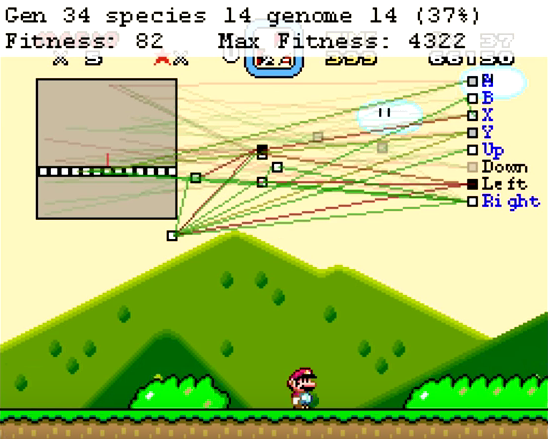
\includegraphics[width=.65\textwidth]{fig/mar-io-example.png}
\caption{\label{fig:mar-io-example}Exemplo da visão do jogo \textit{Super
Mario World} através do projeto \textit{MarI/O}, mostrando elementos de
controle usados pelo NEAT, como a rede neural, as possíveis ações, as
gerações, as especies, os genomas, entre outros.}
\end{figure}

O \textit{MarI/O} é especialmente interessante e relevante porque tem um
objetivo muito similar ao deste trabalho: criar uma inteligência artificial
capaz de jogar uma partida de um jogo. Contudo, existe uma diferença muito
impactante entre \textit{Super Mario World} e \textit{Spelunky} que dificulta a
criação de um \textit{bot}. Em \textit{Super Mario World}, o nível é sempre o
mesmo, o que torna mais fácil medir o desempenho de um \textit{bot}, pois a
disposição do nível é sempre a mesma e a saída sempre se encontra no mesmo
lugar. Além disso, os níveis de \textit{Super Mario World} são essencialmente
horizontais, e movimentar o personagem para a direita quase sempre garante
alguma forma de progresso. Isto facilita ainda mais o processo de treinamento
dos \textit{bots}. Em \textit{Spelunky} não é possível saber de antemão onde se
encontra a saída do nível e o movimento horizontal não garante o progresso,
visto que os níveis não são essencialmente horizontais.
